\chapter{Evaluating Cloudbreak}\label{chap_cloudbreak_eval}

In this chapter we evaluate Cloudbreak and compare its accuracy, runtime, and additional features to a variety of other popular tools. We begin by defining some of the methods and parameters of our tests, and then describe experiments we have done simulated data and two real data sets. Finally, we explore the runtime characteristics of the various tools and the extent to which they can be parallelized.

\section{Evaluation Methods}

\subsection{Choice of SV Detection Tools to Compare To}

We compared the performance of Cloudbreak for detecting deletions and insertions to a selection of popular tools: BreakDancer~\cite{Chen:2009p3}, GASVPro~\cite{Sindi:2012kk}, Pindel~\cite{Ye:2009p2}, and DELLY~\cite{Rausch:2012he}. BreakDancer and Pindel are two of the most highly cited SV detection tools, representing classic RP-based methods and SR-based methods, respectively. GASVPro is a newer hybrid RP method that integrates RD signals and ambiguous mappings into and RP framework based on discordant pairs. DELLY is a more recent hybrid RP-SR method that uses split-read mapping to refine candidate calls made with RP information. DELLY produces two sets of calls, one based solely on RP signals, and the other based on RP calls that could be supported by SR evidence; we refer to these sets of calls as DELLY-RP and DELLY-SR. We also attempted to evaluate MoDIL on the same data given that it is the most algorithmically similar method to Cloudbreak. All of these methods detect deletions. Insertions can be detected by BreakDancer, Pindel, and MoDIL. 

\subsection{Simulated and Biological Data Sets}

As has been observed elsewhere, there is no available test set of real Illumina sequencing data from a sample that has a complete annotation of structural variations from the reference. Therefore, testing with simulated data is important to fully characterize an algorithm's performance characteristics. On the other hand, it is important that the simulated data contain realistic SVs that follow patterns of SVs observed in real data. To address this, we took one of the most complete lists of SVs from a single sample available, the list of homozygous insertions and deletions from the genome of J. Craig Venter~\cite{Levy:2007fb}. Using these variants, we simulated a 30X read coverage data set for a diploid human Chromosome 2 with a mix of homozygous and heterozygous variants.  Since there are relatively few heterozygous insertions and deletions annotated in the Venter genome, we used the set of homozygous indels contained in the HuRef data (\texttt{HuRef.homozygous\_indels.061109.gff}) and randomly assigned each variant to be either homozygous or heterozygous. Based on this genotype, we applied each variant to one or both of two copies of the human GRCh36 chromosome 2 reference sequence. We then simulated paired Illumina reads from these modified references using \emph{dwgsim} from the DNAA software package \cite{DNAA}. We simulated 100bp reads with a mean fragment size of 300bp and a standard deviation of 30bp, and generated 15X coverage for each modified sequence. Pooling the reads from both simulations gives 30X coverage for a diploid sample with a mix of homozygous and heterozygous insertions and deletions.

We downloaded a data set of reads taken from a DNA sample of Yoruban individual NA18507, experiment ERX009609 from the Sequence Read Archive. This sample was sequenced on the Illumina Genome Analyzer II platform with 100bp paired end reads and a mean fragment size (minus adapters) of 300bp, with a standard deviation of 15bp, to a depth of approximately 37X coverage.

To create a gold standard set of insertions and deletions to test against, we pooled annotated variants discovered by three previous studies on the same sample. These included data from the Human Genome Structural Variation Project reported by~\cite{Kidd:2008p926}, a survey of small indels conducted by~\cite{Mills:2011fi}, and insertions and deletions from the merged call set of the phase 1 release of the 1000 Genomes Project~\cite{GenomesProjectConsortium:2012co} which were genotyped as present in NA18507. We merged any overlapping calls of the same type into the region spanned by their unions. It should be noted that the 1000 Genomes call set was partially produced using DELLY and BreakDancer, and therefore those calls are ones that those tools are sensitive to, biasing this test in their favor.

\subsection{Parameters Used for Alignment and SV Detection}

We aligned simulated reads to hg18 chromosome 2, NA18507 reads to the hg19 assembly. Alignments for all programs, unless otherwise noted, were found using BWA \texttt{aln} version 0.6.2-r126, with parameter \texttt{-e 5} to allow for longer gaps in alignments due to the number of small indels near the ends of larger indels in the Venter data set. We also tested the effect of including multiple possible mapping locations for ambiguously mapped reads in results reported in Section~\ref{section_multiple_mappings_eval}. For those tests, we used two different sets of reads with multiple mapping locations reported. The first used alignments generated with BWA in paired-end mode, reporting up to 25 additional hits for each mapping  using the \texttt{-n} and \texttt{-N} parameters for \texttt{bwa sampe} and the script \texttt{xa2multi.pl}. For the second, we attempted to generate an exhaustive list of possible mapping locations by running the GEM aligner in single-ended mode on each read in each pair individually, reporting up to 1000 additional hits per alignment. GEM was executed in parallel using Hadoop tasks which wrap GEM version 1.362 (beta), with parameters \texttt{-e 6 -m 6 -s 2 -q ignore -d 1000 --max-big-indel-length 0}. These parameters request all hits for a read that are within an edit distance of 6 of the reference, within 2 strata of the best hit, with a maximum of 1000 possible alignments reported for each read. GASVPro also accepts ambiguous mappings but expects them to be realigned with a more sensitive alignment tool; we extracted read pairs that did not align concordantly with BWA and re-aligned them with Novoalign V2.08.01, with parameters \texttt{-a -r -Ex 1100 -t 250}. 

We ran BreakDancer version 1.1\_2011\_02\_21 in single threaded mode by first executing \texttt{bam2cfg.pl} and then running \texttt{breakdancer\_max} with the default parameter values.  To run BreakDancer in parallel mode we first ran \texttt{bam2cfg.pl} and then launched parallel instances of \texttt{breakdancer\_max} for each chromosome using the \texttt{-o} parameter. We ran DELLY version 0.0.9 with the \texttt{-p} parameter and default values for other parameters. For the parallel run of DELLY we first split the original BAM file with BamTools \cite{Barnett:2011hm}, and then ran instances of DELLY in parallel for each BAM file. We ran GASVPro version 1.2 using the \texttt{GASVPro.sh} script and default parameters. Pindel 0.2.4t was executed with default parameters in single CPU mode, and executed in parallel mode for each chromosome using the \texttt{-c} option. We executed MoDIL with default parameters except for a \texttt{MAX\_DEL\_SIZE} of 25000, and processed it in parallel on our cluster with a step size of 121475. To execute parallelize other SV detection tools we wrote simple scripts to submit jobs to the cluster using the HTCondor scheduling engine \cite{condor-practice} with directed acyclic graphs to describe dependencies between jobs. 

\subsection{SV Prediction Evaluation}\label{section_prediction_evaluation}

Due to the inability of most tools to determine the exact breakpoint coordinates of an SV given read pair data, as well as the potential for uncertaintly due to error in real gold standard data sets, it is necessary to define a rule for determining whether or not a predicted SV call is correct or not. There are many ways of doing so, each with their own characteristics. For example, the authors of BreakDancer~\cite{Chen:2009p3} and VariationHunter~\cite{Hormozdiari:2009p284} considered a predicted deletion to be correct if had a 50\% reciprocal overlap with a deletion in the test set. For GASVPro~\cite{Sindi:2012kk}, Sindi et al. defined a ``double uncertainty'' metric, in which tolerance parameters $\epsilon$ and $\delta$ could be defined for the predictions and for the test set respectively, and a deletion prediction of the interval $[x,y]$ is deemed to be correct if there exists an interval in the test set $[a,b]$ for which there is overlap between both pairs of intervals $\langle[x-\epsilon,x+\epsilon]$,$[a-\delta,a+\delta]\rangle$ and $\langle[y-\epsilon,y+\epsilon]$,$[b-\delta,b+\delta]\rangle$. The forthcoming SMASH~\cite{2013arXiv1310.8420T} benchmark of variant callers, including SV detection tools, counted a deletion call as a match if the left breakpoint of the call was within 100bp of the left breakpoint of the deletion interval in the test set and the difference between lengths of the two intervals was less than or equal to 100bp. The authors of the iSVP pipeline~\cite{Mimori:2013wx}, meanwhile, assigned a quality score between 0 and 1 based on the ratio of the length of the intersection of the predicted and test variants, with 50bp margins added to each, to the length of the union of the two intervals. 

To evaluate Cloudbreak we decided to use looser standards for calling a prediction true, because we would like to test the maximum potential sensitivity of the algorithmic approach even if the resolution of the breakpoints is limited. We feel that this is appropriate given that most calls from SV detection tools will likely be validated either through an additional computational step such as local assembly, or through wet lab techniques such as PCR. Therefore, we use the following criteria to define a true prediction given a gold standard set of deletion and insertion variants to test against: A predicted deletion is counted as a true positive if a) it overlaps with a deletion from the gold standard set, b) the length of the predicted call is within 300bp (the library fragment size in both our real and simulated libraries) of the length of the true deletion, and c) the true deletion has not been already been discovered by another prediction from the same method. For evaluating insertions, each algorithm produces insertion predictions that define an interval in which the insertion is predicted to have occurred with start and end coordinates $s$ and $e$ as well as the predicted length of the insertion, $l$. The true insertions are defined in terms of their actual insertion coordinate $i$ and their actual length $l_a$. Given this information, we modify the overlap criteria in a) to include overlaps of the intervals $\langle s,\max{\left(e,s+l\right)} \rangle$ and $\langle i,i+l_a \rangle$. In this study we are interested in detecting events larger than 40bp, because with longer reads, smaller events can be more easily discovered by examining gaps in individual reads. Both Pindel and MoDIL make many calls with a predicted event size of under 40bp, so we remove those calls from the output sets of those programs. Finally, we exclude from consideration calls from all approaches that match a true deletion of less than 40bp where the predicted variant length is less than or equal to 75bp in length.

\section{Results on Simulated Data}

\subsection{Accuracy and Runtime}

\begin{figure}
\centering
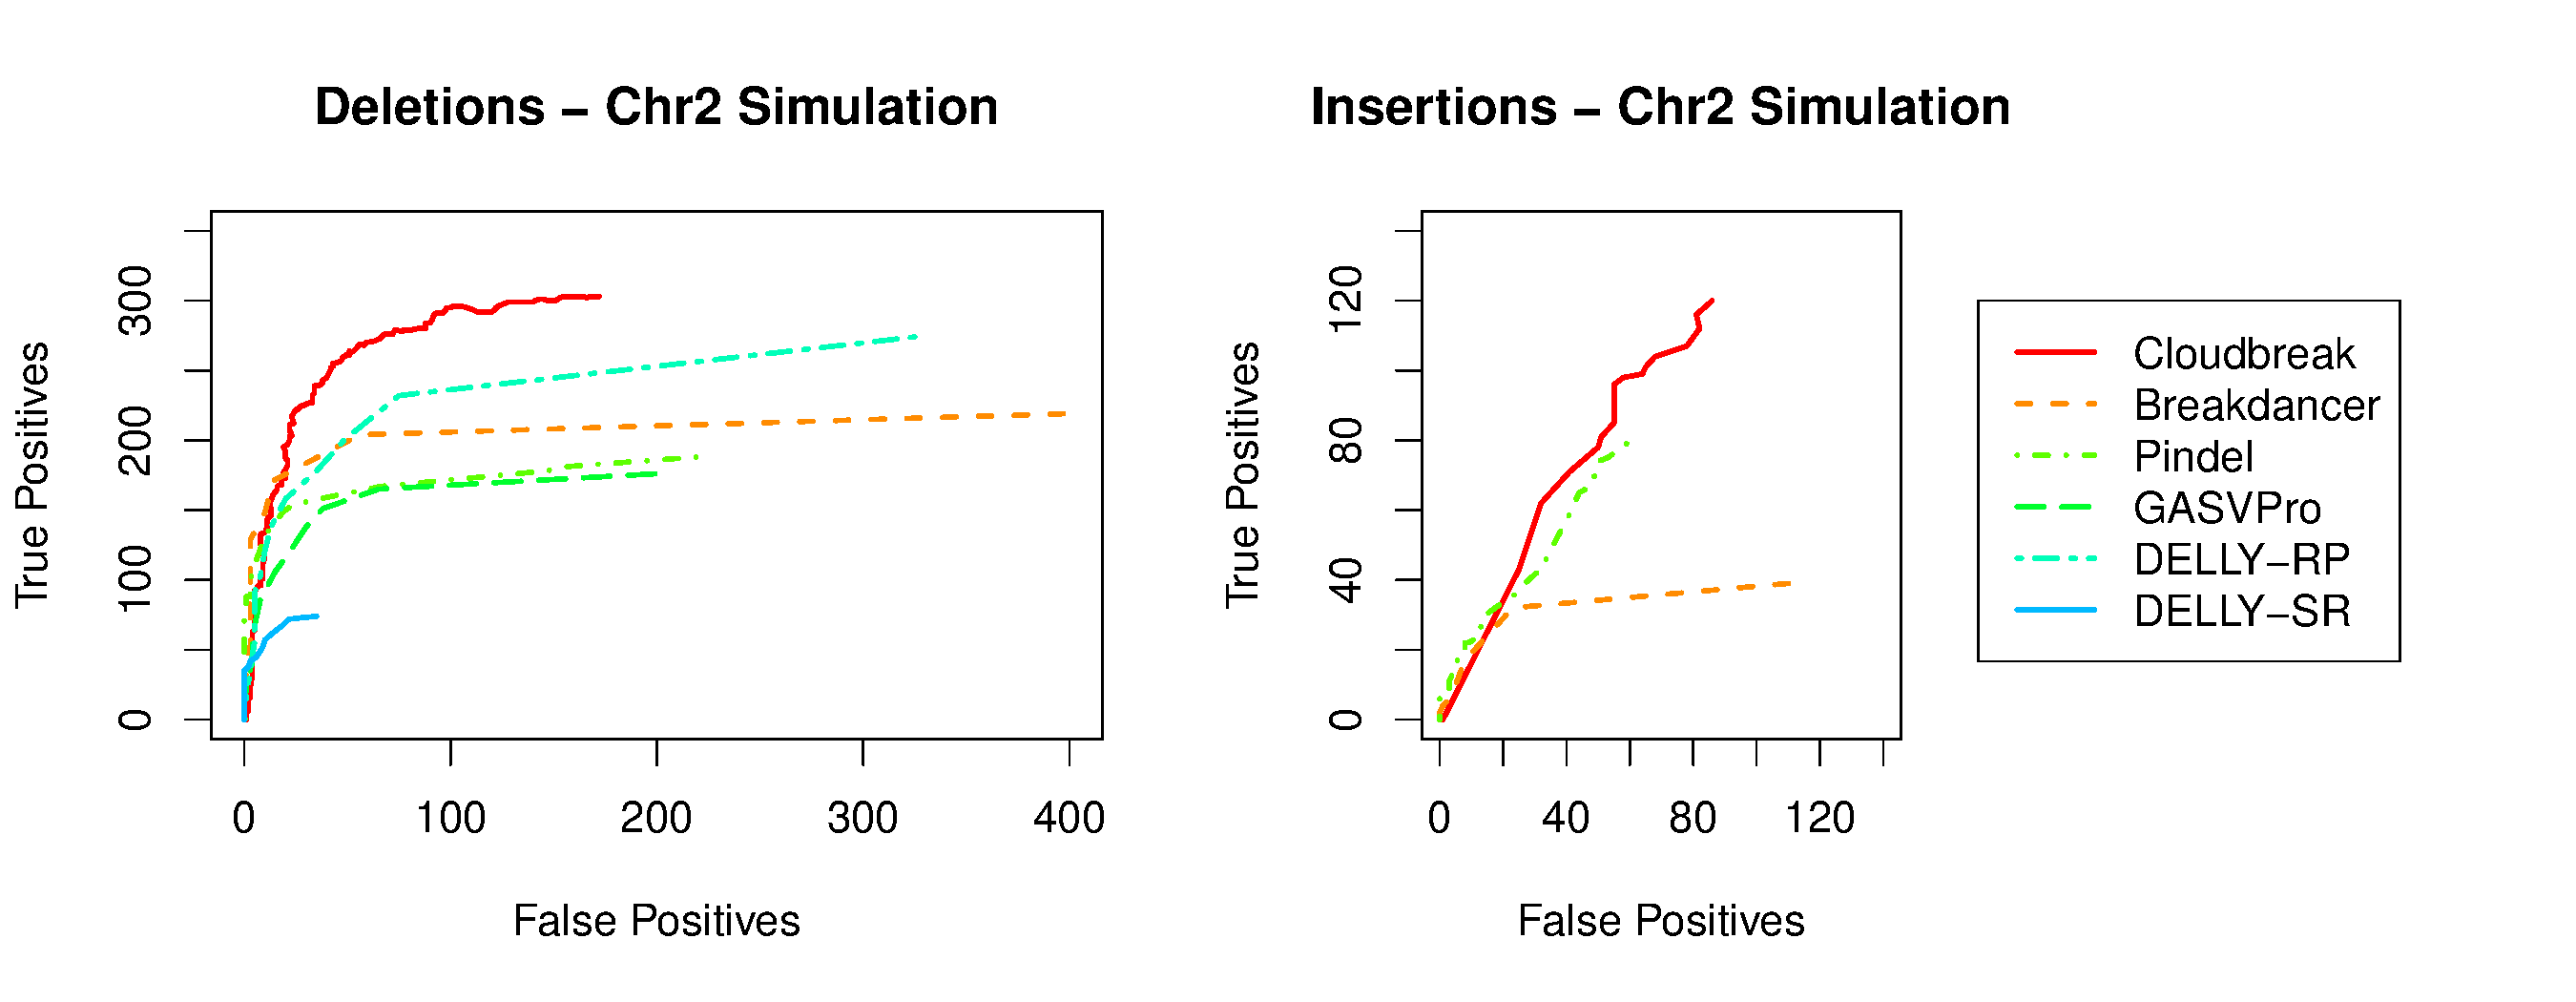
\includegraphics[width=1\textwidth]{figures/CHR2SIM_ROC_COMBINED_ROCS_POSTER.pdf}
\caption{Accuracy and runtime performance on a simulated data set. Receiver Operating Characteristic (ROC) curves showing the specificity and sensitivity of each tool to deletions and insertions larger than 40bp on a simulated set of reads giving diploid coverage of 30X on human chromosome 2. Deletions and insertions from the Venter genome were randomly added to one or both haplotypes. Each point on a curve represents a different threshold on the confidence of predictions made by that tool. Thresholds vary by: Cloudbreak - likelihood ratio; BreakDancer, DELLY, GASVPro - number of supporting read pairs; Pindel - simple score.}
\label{chr2CombinedRoc}
\end{figure}

Figure~\ref{chr2CombinedRoc} shows Receiver Operating Characteristics (ROC) curves of the performance of each algorithm for detecting deletions and insertions on the simulated data set. See Section~\ref{section_prediction_evaluation} for a description of how we identified correct predictions. All approaches show excellent specificity at high thresholds in this simulation. Cloudbreak provides the greatest specificity for deletions at higher levels of sensitivity, followed by DELLY. For insertions, Cloudbreak clearly provides the best combinations of sensitivity and specificity. Figure~\ref{chr2BestRuntimes} shows the runtimes for each tool on the simulated data set, parallelized when possible. Runtimes exlude alignment, which should be similar for all tools. Cloudbreak's runtime is half that of BreakDancer, the next fastest tool, processing the simulated data in under six minutes. Of course, Cloudbreak uses many more CPUs as a distributed algorithm. See Section~\ref{section_comparing_runtime} for a more detailed discussion of runtimes and the amount of parallelization that was done for each tool. The output which we obtained from MoDIL did not have a threshold that could be varied to correlate with the trade-off between precision and recall and therefore it is not included in ROC curves; in addition, MoDIL ran for 52,547 seconds using 250 CPUs in our cluster, so results are not included in the runtime figure. Apart from the alignment phase, which is embarrassingly parallel, the feature generation job is the most computationally intensive part of the Cloudbreak workflow. Therefore, to test the algorithm's scalability we measured the runtime of that job on Hadoop clusters made up of varying numbers of nodes and observed that linear speedups can be achieved in this portion of the algorithm by adding additional nodes to the cluster until a point of diminishing returns is reached (Figure~\ref{scalability}).

\begin{figure}
\centering
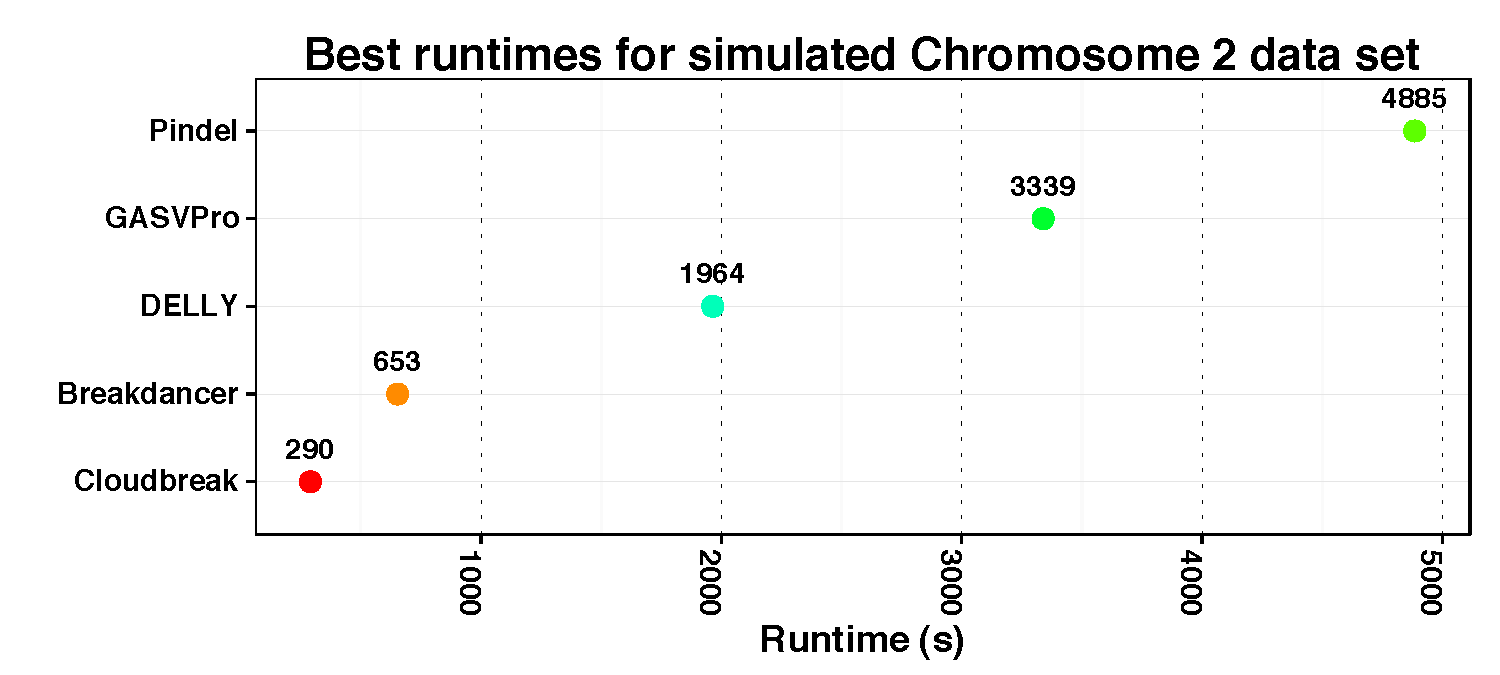
\includegraphics[width=1\textwidth]{figures/chr2BestRuntimes_horizontal.pdf}
\caption{Runtimes for each tool on the simulated data set, not including alignment time, parallelized when possible. See Section~\ref{section_comparing_runtime} for details on measuring and parallelizing the runtime of each tool.}
\label{chr2BestRuntimes}
\end{figure}

\begin{figure}
\centering
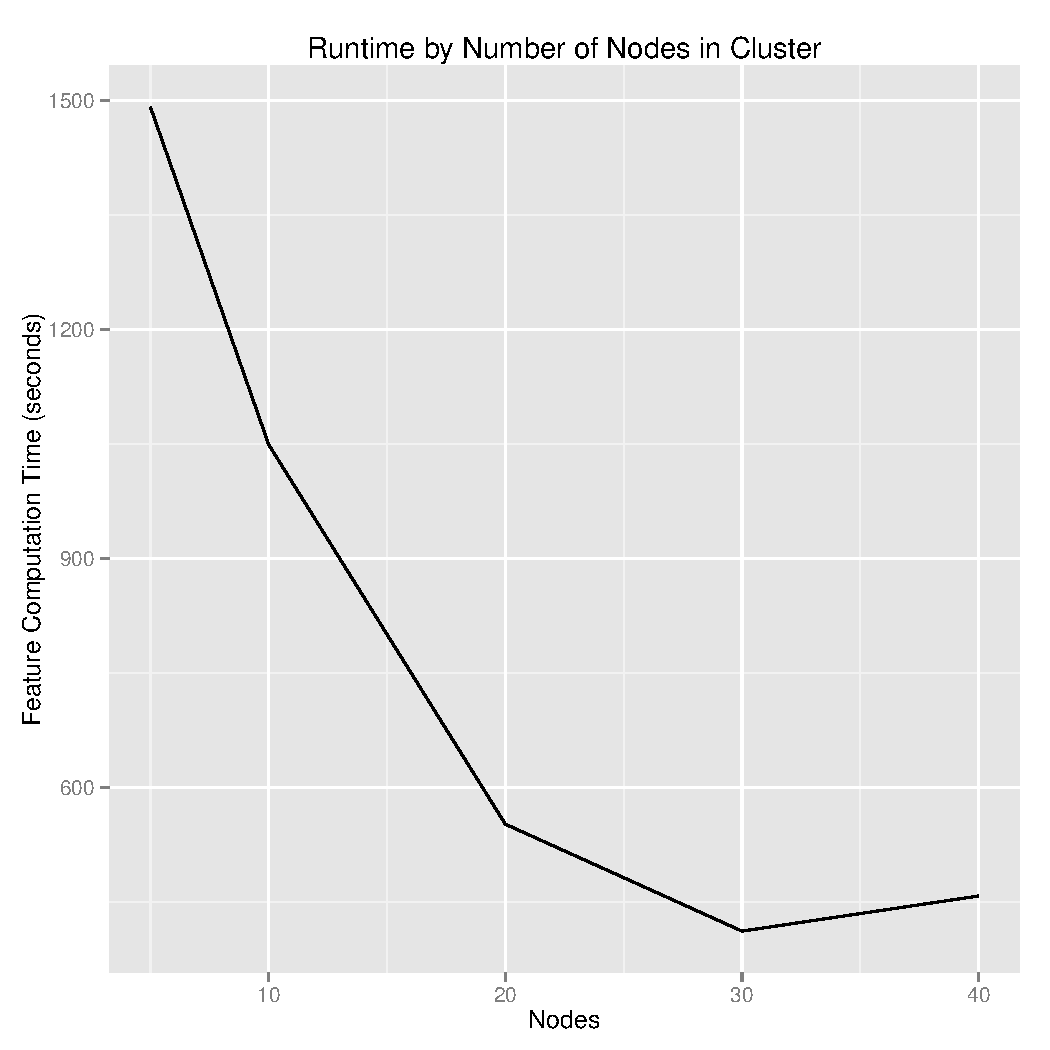
\includegraphics[width=.8\textwidth]{/Users/cwhelan/Documents/svpipeline/figures/runtimeByNodes.pdf}
\caption{Scalability of the Cloudbreak algorithm. Runtime of the Cloudbreak feature generation job for the simulated Chromosome 2 data is shown on Hadoop clusters consisting of varying numbers of compute nodes. Clusters were created in the Amazon Elastic Compute Cloud.}
\label{scalability}
\end{figure}

Choosing the correct operating point or threshold to set on the output of an SV calling algorithm can be difficult when operating on a new data set. The use of simulated data and ROC curves allows for some investigation of the performance characteristics of algorithms at varying levels. First, we characterized the predictions made by each algorithm at the operating point which gives them maximum sensitivity. For Cloudbreak we chose an operating point at which marginal improvements in sensitivity became very low. The results for both deletion and insertion predictions are summarized in Table~\ref{chr2DeletionAndInsertionPredsMaxSensitivity}. MoDIL and Cloudbreak exhibited the greatest recall for deletions. Cloudbreak has high precision and recall for deletions at this threshold, and discovers many more small deletions. For insertions, Cloudbreak has the highest recall, although recall is low for all four approaches. Cloudbreak again identifies the most small variants. Pindel is the only tool which can consistently identify large insertions, as insertions larger than the library insert size do not produce mapping signatures detectable by read-pair mapping. 

\begin{table}
\begin{center}
\resizebox{\textwidth}{!}{
\begin{tabular}{r|rrrr|rrrrr}
  \cline{2-10}
   &                     & Prec. & Recall & F1 & 40-100bp  & 101-250bp  & 251-500bp & 501-1000bp & $>$ 1000bp \\ 
\hline
\multirow{7}{*}{\begin{sideways}Deletions\end{sideways}} & Total Number &          &           &  &  224 &  84 & 82 &  31 & 26\\ 
  \hline
\cline{2-10}
&  Cloudbreak    &  0.638 & \textbf{0.678} & \textbf{0.657} & \textbf{153} (9)  & 61 (0) &  62 (0) & 12 (0) & 15 (0) \\ 
&  BreakDancer   &  0.356 & 0.49 & 0.412 & 89 (0)  & 54 (0) &  53 (0) & 8 (0) & 15 (0) \\ 
&  GASVPro        & 0.146 & 0.432 & 0.218 & 83 (2)  & 32 (0) &  55 (0) & 8 (0) & 15 (0) \\ 
&  DELLY-RP           & 0.457 & 0.613 & 0.613 & 114 (3)  & \textbf{68} (0) &  \textbf{66} (0) & 9 (1) & 17 (0) \\ 
&  DELLY-SR           & \textbf{0.679} & 0.166 &  0.266 & 0 (0)  & 3 (0) &  49 (0) & 6 (0) & 16 (0) \\ 
&  Pindel           & 0.462 & 0.421 &  0.44 & 96 (\textbf{11})  & 24 (0) &  48 (0) & 5 (0) & 15 (0)\\ 
&  MoDIL           & 0.132  & 0.66 & 0.22 & 123 (6)  & 66 (\textbf{3}) &  \textbf{66} (\textbf{11}) & \textbf{17} (\textbf{7}) & \textbf{23} (\textbf{8})\\ 
   \hline
\multirow{5}{*}{\begin{sideways}Insertions\end{sideways}} & Total Number &          &           & & 199 &  83 & 79 &  21 & 21\\ 
\cline{2-10}
&  Cloudbreak   &0.451 & \textbf{0.305}  & \textbf{0.364}  & \textbf{79} (\textbf{32})  & \textbf{32} (\textbf{18}) &  \textbf{11} (8) & 1 (0) & 0 (0) \\ 
&  BreakDancer & 0.262 & 0.0968  & 0.141  & 23 (5)  & 14 (5) &  2 (1) & 0 (0) & 0 (0) \\ 
&  Pindel          & \textbf{0.572} & 0.196 &  0.292 & 52 (25)  & 5 (1) &  10 (\textbf{9}) & \textbf{3} (\textbf{2}) & \textbf{9} (\textbf{9})\\ 
&  MoDIL          & 0.186 & 0.0521 &  0.0814 & 14 (1)  & 4 (0) &  1 (0) & 2 (\textbf{2}) & 0 (0)\\ 
\hline
\end{tabular}}
\end{center}
\caption{The number of simulated deletions and insertions in the 30X diploid chromosome 2 with Venter indels found by each tool at maximum sensitivity, as well as the number of those variants that were discovered exclusively by each tool (in parentheses). The total number of variants in each size class in the true set of deletions and insertions is shown in the first row of each section.}
\label{chr2DeletionAndInsertionPredsMaxSensitivity}
\end{table}

We also used the ROC curves to attempt to characterize the predictions made by each algorithm when a low false discovery rate is required. Table~\ref{chr2DeletionPredsFDR10} shows the total number of simulated deletions found by each tool when choosing a threshold that gives an FDR closest to 10\% based on the ROC curve. At this more stringent threshold, Cloudbreak identifies more deletions in every size category than any other tool. Performance on insertions never reached an FDR of 10\% for any threshold, so insertion predictions are not included in this table. 

\begin{table}
\begin{center}
\begin{tabular}{rrrrrr}
 \hline
 & 40-100bp & 101-250bp & 251-500bp & 501-1000bp & $>$ 1000bp \\ 
 Total Number & 224 & 84 & 82 & 31 & 26\\ 
 \hline
 Cloudbreak & \textbf{68} (17) & \textbf{67} (\textbf{10}) & \textbf{56} (\textbf{5}) & \textbf{11} (\textbf{3}) & \textbf{15} (\textbf{0}) \\ 
 BreakDancer & 52 (8) & 49 (2) & 49 (0) & 7 (0) & 14 (\textbf{0}) \\ 
 GASVPro  & 35 (2) & 26 (0) & 26 (0) & 2 (0) & 6 (\textbf{0}) \\ 
 DELLY-RP  & 22 (1) & 56 (1) & 40 (0) & 8 (0) & 12 (\textbf{0}) \\ 
 DELLY-SR  & 0 (0) & 2 (0) & 28 (0) & 2 (0) & 10 (\textbf{0}) \\ 
 Pindel  & 60 (\textbf{32}) & 16 (0) & 41 (2) & 1 (0) & 12 (\textbf{0})\\ 
 \hline
\end{tabular}
\end{center}
\caption{The number of simulated deletions in the 30X diploid chromosome 2 with Venter indels found by each tool at a 10\% FDR, as well as the number of those deletions that were discovered exclusively by each tool (in parentheses). The total number of deletions in each size class in the true set of deletions is shown in the second row of the header.}
\label{chr2DeletionPredsFDR10}
\end{table}

\subsection{Choice of Window Size}\label{section_window_size}

A key parameter choice for Cloudbreak is the size of the fixed-width, non-overlapping windows used for local feature computation. The experiments reported in this Chapter all used a window size of 25bp. Using the simulated data set, we evaluated the effect of choosing differing window sizes on runtime, breakpoint resolution, and accuracy. Figure~\ref{figure_runtime_by_window_size} shows the runtime of the feature computation and variant calling steps of Cloudbreak on the Chromosome 2 data set using differing window sizes. Runtime decreases dramatically with larger window sizes. For very small window sizes, the runtime is dominated by the variant extraction job, which is only parallelized by chromosome and therefore only runs on one core when running on the simulated data set. Table~\ref{chr2AccuracyByWindowSize} shows several accuracy measures for Cloudbreak running with varying window sizes, using the same threshold for each run. The greatest recall is achieved at very low window sizes, probably because evidence for smaller variants is less likely to be mixed in with non-variant supporting read pairs from the flanking regions. However, overall accuracy is high until window sizes reach 50bp, at which point recall decreases dramatically. Finally, we examined the effect of breakpoint accuracy on window size and found that it had little effect (Figure~\ref{breakpoint_resolution_by_windowSize}).

\begin{figure}
\centering
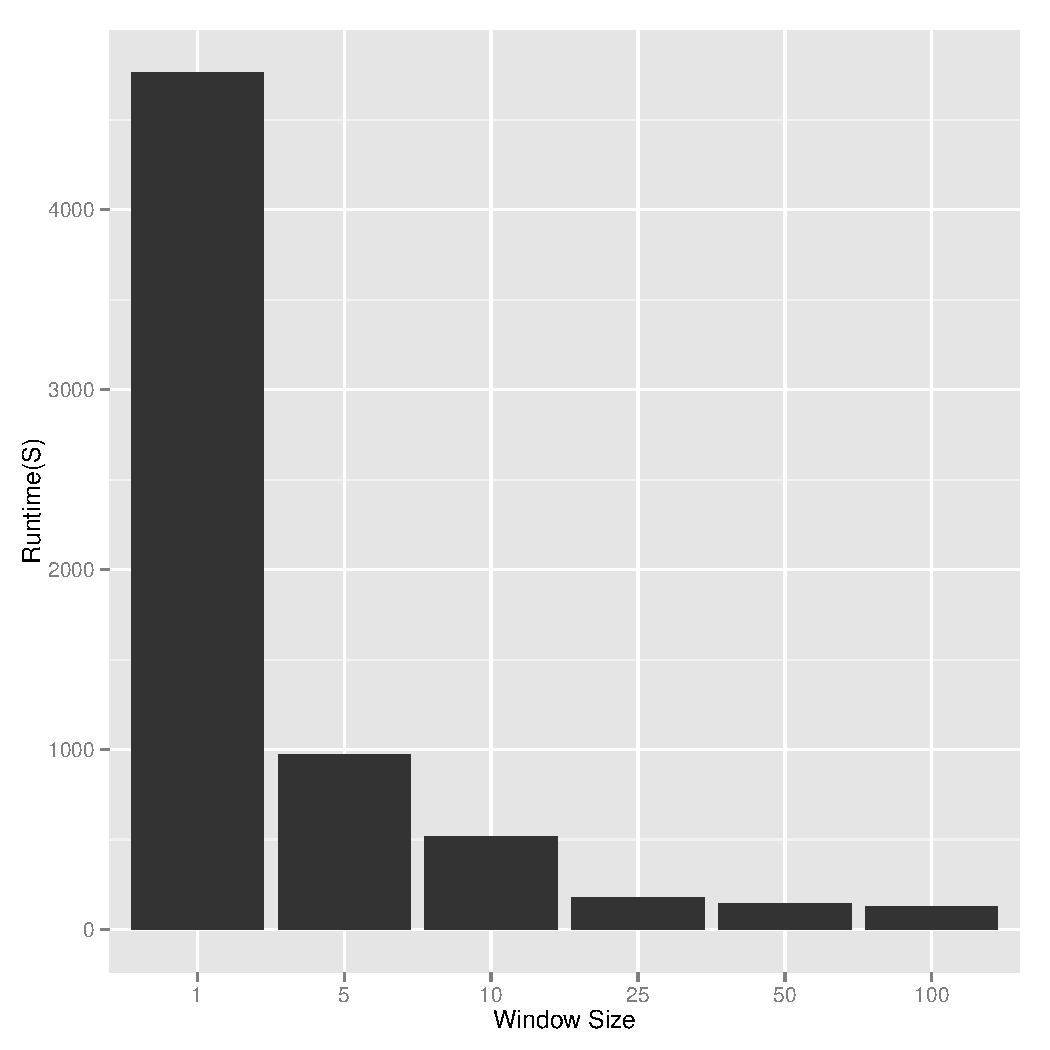
\includegraphics[width=.8\textwidth]{figures/runtime_by_windowSize.pdf}
\caption{Runtimes for Cloudbreak on the Chromosome 2 simulated data set using differing choices of window size. Runtimes include the feature computation and variant calling Cloudbreak Hadoop jobs.}
\label{figure_runtime_by_window_size}
\end{figure}

\begin{table}
\begin{center}
\begin{tabular}{r|rrrrr}
 \hline
 Window Size & Calls & True Positives & Precision & Recall & F1 \\ 
 \hline
   1 & 274 & 228 & 0.832 & 0.57 & 0.677 \\ 
   5 & 268 & 228 & 0.851 & 0.57 & 0.683 \\ 
   10 & 258 & 223 & 0.864 & 0.557 & 0.678 \\ 
   25 & 240 & 217 & 0.904 & 0.542 & 0.678 \\ 
   50 & 215 & 194 & 0.902 & 0.485 & 0.631 \\ 
   100 & 162 & 141 & 0.87 & 0.352 & 0.502 \\  
\end{tabular}
\end{center}
\caption{Accuracy measures for Cloudbreak on the Chromosome 2 simulated data set using different choices of window size. For each window size the same Cloudbreak score threshold was used (1.98).}
\label{chr2AccuracyByWindowSize}
\end{table}
\begin{figure}
\centering
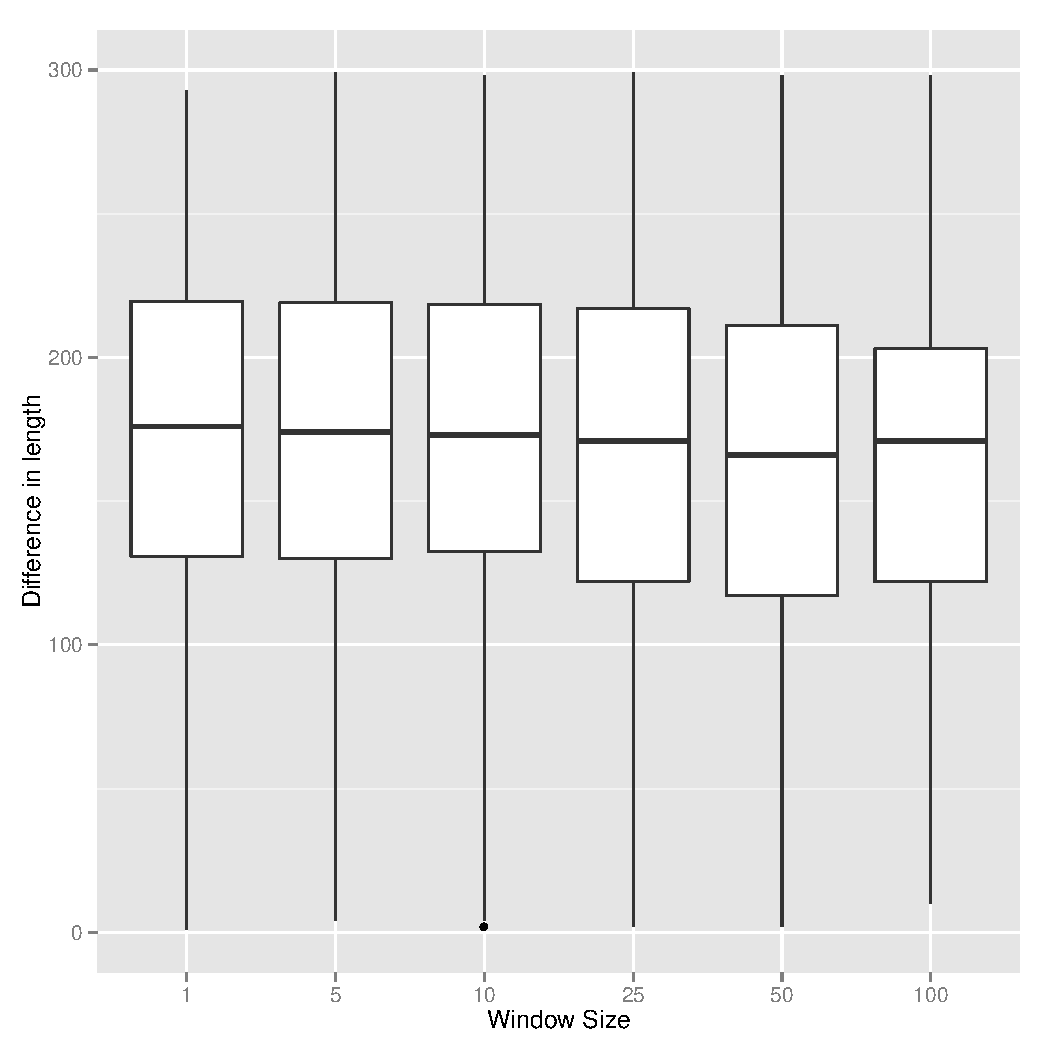
\includegraphics[width=.8\textwidth]{figures/breakpoint_resolution_by_windowSize.pdf}
\caption{Breakpoint resolution for Cloudbreak on the Chromosome 2 simulated data set using differing choices of window size.}
\label{breakpoint_resolution_by_windowSize}
\end{figure}

\section{Results on Biological Data}\label{section_na18507}

\subsection{Accuracy and Runtime}

\begin{figure}
\centering
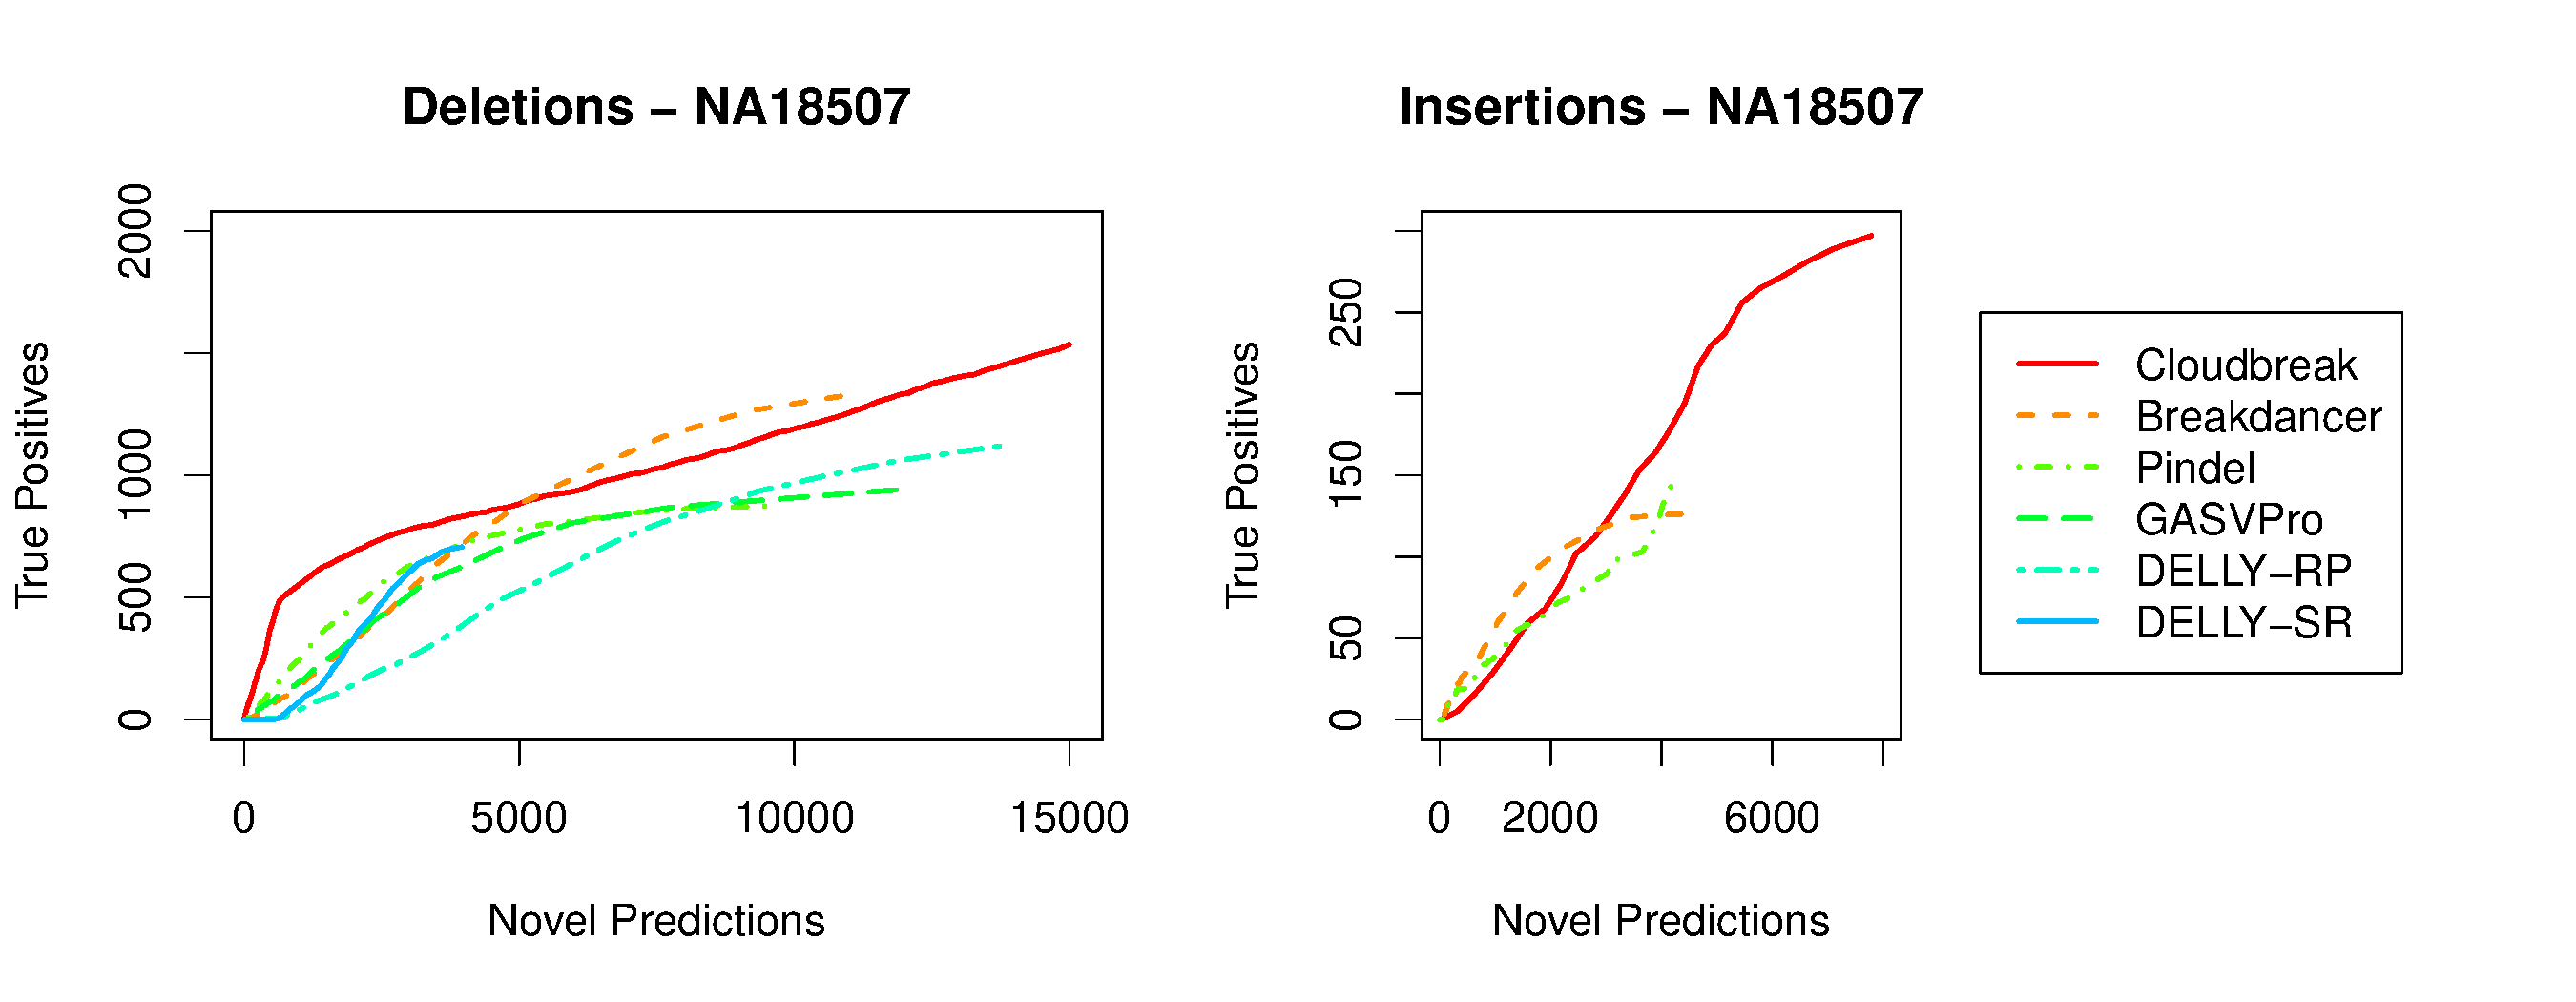
\includegraphics[width=1\textwidth]{figures/NA18507_COMBINED_ROCS_POSTER.pdf}
\caption{Accuracy on the 37X NA18507 sample. ROC curves for deletion and insertion prediction performance, tested against the combined gold standard sets of deletions taken from~\cite{Kidd:2008p926},~\cite{Mills:2011fi}, and~\cite{GenomesProjectConsortium:2012co}.}
\label{NA18507CombinedRoc}
\end{figure}

Figure~\ref{NA18507CombinedRoc} shows the performance of each algorithm on the NA18507 data set when compared against the gold standard set for both deletions and insertions. We were unable to run MoDIL on the whole-genome data set due to the estimated runtime and storage requirements. All other algorithms show far less specificity for the gold standard set than they did for the true variants in the single chromosome simulation, although it is difficult to tell how much of the difference is due to the added complexity of real data and a whole genome, and how much is due to missing variants in the gold standard set that are actually present in the sample. For deletions, Cloudbreak is the best performer at the most stringent thresholds, and has the highest or second highest precision at higher sensitivity levels. Cloudbreak has slightly lower accuracy for insertions than the other tools at more stringent thresholds, although it can identify the most variants at higher levels of sensitivity. Figure~\ref{NA18507BestRuntimes} and Table~\ref{runtimes} show the runtime of each of the tools on the NA18507 dataset. Cloudbreak processes the sample in under 15 minutes on our cluster, more than six times as fast as the next fastest program, BreakDancer, even when BreakDancer is run in parallel for each chromosome on different nodes in the cluster.

\begin{figure}
\centering
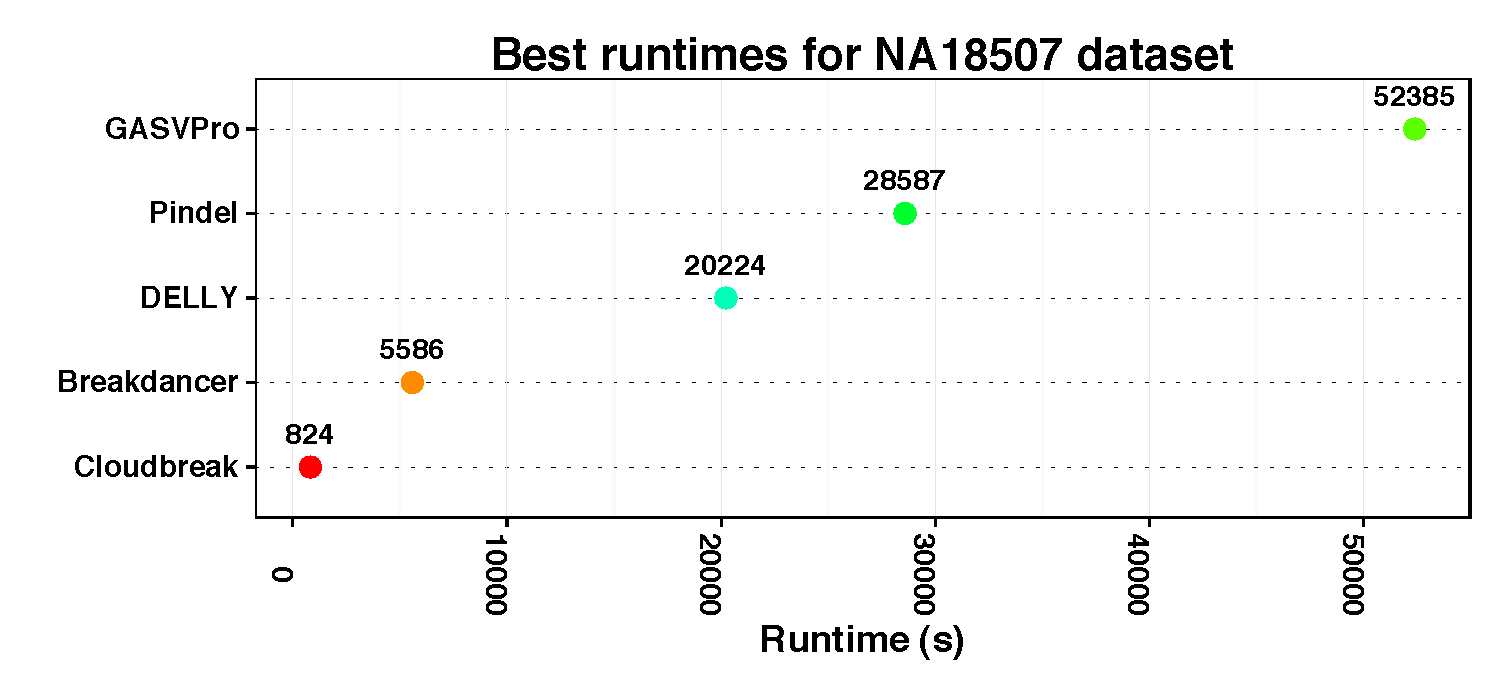
\includegraphics[width=1\textwidth]{figures/NA18507BestRuntimes_horizontal.pdf}
\caption{Runtimes for each tool on the NA18507 data set, not including alignment time, parallelized when possible. See Section~\ref{section_comparing_runtime} for details on measuring and parallelizing the runtime of each tool.}
\label{NA18507BestRuntimes}
\end{figure}

Given the high number of false positives produced by all tools at maximum sensitivity indicated by the ROC curves, we decided to characterize the predictions made by each tool at more stringent thresholds. We examined the deletion predictions made by each algorithm using the same cutoffs that yielded a 10\% FDR on the simulated chromosome 2 data set, adjusted proportionally for the difference in coverage from 30X to 37X. For insertions, again, we were forced to use the thresholds that gave maximum sensitivity for each tool due to the high observed FDR rates in the simulated data. The precision and recall at these thresholds with respect to the gold standard set, as well as the performance of each algorithm at predicting variants of each size class at those thresholds, is shown in Table~\ref{NA18507DeletionAndInsertionPreds}. For deletions, Cloudbreak has the greatest sensitivity of any tool at these thresholds, identifying the most variants in each size class. Pindel exhibits the highest precision with respect to the gold standard set. For insertions, Pindel again has the highest precision at maximum sensitivity, although according the ROC curve it is possible to choose a threshold for Cloudbreak with higher precision and recall. At maximum sensitivity, Cloudbreak identifies 120 more insertions from the gold standard set than Pindel, giving it by far the highest recall.

\begin{table}
\begin{center}
\resizebox{\textwidth}{!}{
\begin{tabular}{r|rrrr|rrrrr}
  \cline{2-10}
&  & Prec. & Recall & F1 & 40-100bp & 101-250bp & 251-500bp & 501-1000bp & $>$ 1000bp \\ 
\hline
\multirow{6}{*}{\begin{sideways}Deletions\end{sideways}} & Total Number & & & & 7,462 & 240 & 232 & 147 & 540 \\
  \hline
\cline{2-10}
& Cloudbreak & 0.0943 & \textbf{0.17} & 0.121 & \textbf{573} (\textbf{277})  & \textbf{176} (\textbf{30}) &  \textbf{197} (\textbf{18}) & \textbf{121} (\textbf{6}) & \textbf{399} (\textbf{24}) \\ 
& BreakDancer & 0.137 & 0.123 &  \textbf{0.13} & 261 (29)  & 136 (3) &  178 (0) & 114 (0) & 371 (0) \\  
&  GASVPro & 0.147 & 0.0474 &  0.0717 & 120 (21)  & 40 (2) &  85 (0) & 36 (0) & 128 (0) \\ 
&  DELLY-RP & 0.0931 & 0.1 &  0.0965 & 143 (6)  & 128 (3) &  167 (1) & 103 (0) & 323 (1) \\ 
&  DELLY-SR & 0.153 & 0.0485 &  0.0736 & 0 (0)  & 26 (0) &  123 (0) & 66 (0) & 203 (0) \\ 
&  Pindel & \textbf{0.179} & 0.0748 &  0.106 & 149 (8)  & 61 (0) &  149 (0) & 69 (1) & 217 (0) \\ 
\hline
\multirow{4}{*}{\begin{sideways}Insertions\end{sideways}} & Total Number & & & & 536 & 114 & 45 & 1 & 0 \\
\cline{2-10}
& Cloudbreak & 0.0323 & \textbf{0.455} &  0.0604 & \textbf{265} (\textbf{104})  & \textbf{49} (\textbf{24}) &  3 (1) & 0 (0)  & 0 (0)  \\ 
& BreakDancer & 0.0281 & 0.181 &  0.0487 & 97 (10)  & 27 (5) &  2 (1) & 0 (0) & 0 (0) \\  
&  Pindel & \textbf{0.0387} & 0.239 &  \textbf{0.0666} & 144 (45)  & 14 (7) &  \textbf{7} (\textbf{6}) & \textbf{1} (\textbf{1}) &  0 (0) \\ 
\hline
\end{tabular}}
\end{center}
\caption{The precision and recall with respect to the gold standard set of deletions and insertions for each tool on the NA18507 data, as well as the number of variants found in each size class found. Exclusive predictions are in parentheses. For deletions, the same cutoffs were used as for the simulated data as in Table~\ref{chr2DeletionPredsFDR10}, adjusted for the difference in coverage from 30X to 37X. For insertions, the maximum sensitivity cutoff was used.}
\label{NA18507DeletionAndInsertionPreds}
\end{table}

\subsection{Breakpoint Resolution}

We expected that the methods tested here would vary in their breakpoint resolution: SR methods can achieve single nucleotide breakpoint resolution, while RP methods depend on insert size evidence from overlapping fragments that will likely not indicate the exact location of the breakpoint. This distinction can be seen clearly in Figure~\ref{breakpoint_resolution}. Cloudbreak has the lowest resolution of any of the RP tools tested, with GASVPro also having relatively poor resolution. Pindel and DELLY-SR, meanwhile, use split read mappings to pinpoint the exact breakpoint correctly in many cases. Cloudbreak's resolution suffers because the independent calculation of features from the distribution of overlapping insert sizes does not allow the algorithm to keep track of the actual coordinates of the mapped reads from each pair, which other tools use to set bounds on the true breakpoint locations. Cloudbreak's goal, however, is to increase sensitivity and specificity to actual variants in the hopes that such calls could still be useful even if their resolution is limited. This seems reasonable to us, especially given the possibility of pipelines in which RP calls are validated \emph{in silico} by local assembly methods or split-read methods.

\begin{figure}
\centering
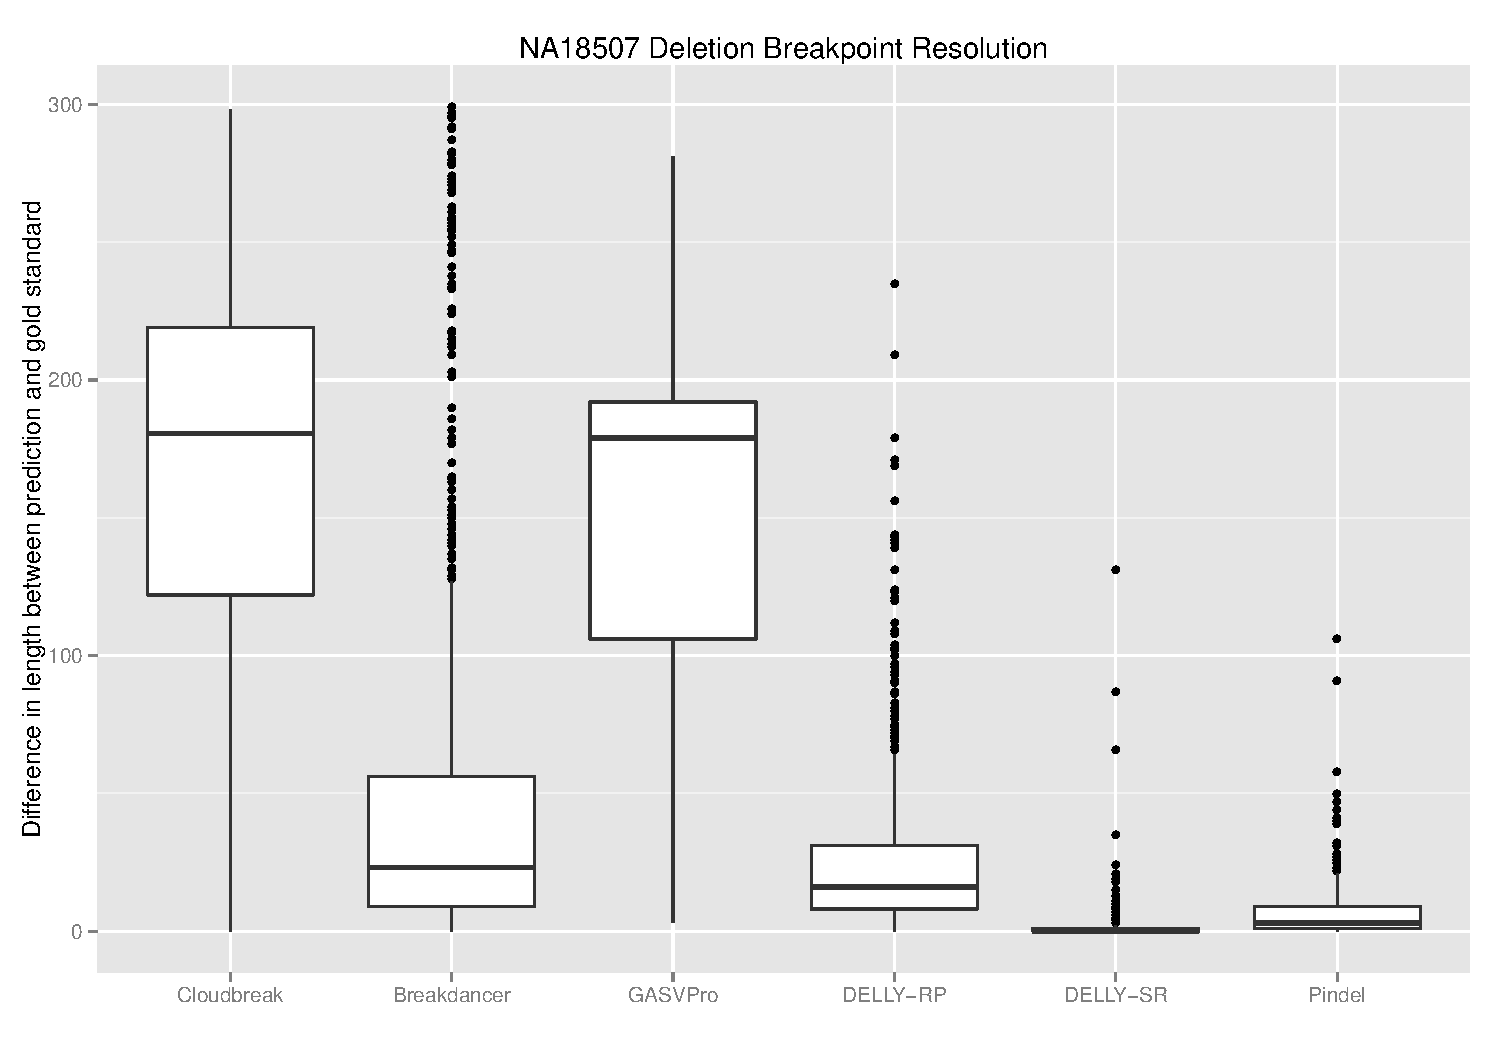
\includegraphics[width=.8\textwidth]{/Users/cwhelan/Documents/svpipeline/figures/breakpointResolutionNA18507.pdf}
\caption{Breakpoint resolution for each tool for deletions from the gold standard set on the NA18507 data. For each correctly predicted deletion, we calculated the difference in length between the true deletion and the prediction.}
\label{breakpoint_resolution}
\end{figure}

\section{Results on a Low-Coverage Cancer Data Set}

We also tested Cloudbreak on the sequencing data set obtained from a patient with acute myeloid leukemia (AML) described in Section~\ref{section_aml_pipeline}. This data set consisted of 76bp paired end reads with a mean insert size of 285bp and standard deviation of 50bp, yielding sequence coverage of 5X and physical coverage of 8X. Using a pipeline consisting of Novoalign, BreakDancer, and a set of custom scripts for filtering and annotating candidate SVs, we had previously identified a set of variants present in this sample and validated several using PCR, including 8 deletions. Cloudbreak was able to identify all 8 of the validated deletions, showing that it is still sensitive to variants even when using lower coverage data sets with a greater variance of insert sizes.

\section{Genotyping Variants}\label{section_genotyping_eval}

Because Cloudbreak explicitly models zygosity in its feature generation algorithm, it can predict the genotypes of identified variants. We tested this on both the simulated and NA18507 data sets. For the NA18507 data set, we considered the deletions from the 1000 Genomes Project, which had been genotyped using the population-scale SV detection algorithm Genome STRiP \cite{Handsaker:2011ki}. Cloudbreak was able to achieve 92.7\% and 95.9\% accuracy in predicting the genotype of the deletions it detected at our 10\% FDR threshold in the simulated and real data sets, respectively. Table~\ref{deletionGenotypeaccuracy} shows confusion matrices for the two samples using this classifier. None of the three input sets that made up the gold standard for NA18507 contained a sufficient number of insertions that met our size threshold and also had genotyping information. Of the 123 insertions detected by Cloudbreak on the simulated data set, 43 were heterozygous. Cloudbreak correctly classified 78 of the 80 homozygous insertions and 31 of the 43 heterozygous insertions, for an overall accuracy of 88.6\%.

\begin{table}
\begin{center}
\resizebox{\textwidth}{!}{
\begin{tabular}{r|r|rr|rr|}
\multicolumn{2}{c}{}  & \multicolumn{4}{c}{Actual Genotypes} \\
\multicolumn{2}{c}{}  & \multicolumn{2}{c}{Simulated Data} & \multicolumn{2}{c}{NA18507} \\
\cline{3-6}
\multicolumn{2}{c|}{} &  Homozygous & Heterozygous & Homozygous & Heterozygous \\ 
\cline{2-6}
\multirow{2}{*}{\shortstack{Predicted \\ Genotypes}} & Homozygous & 35 & 2 &  96 & 21 \\
 & Heterozygous & 0 & 39 &  2 & 448 \\
\cline{2-6}
\end{tabular}
}
\end{center}
\caption{Confusion matrices for the predicted genotype of deletions found by Cloudbreak on both the simulated and NA18507 data sets.}
\label{deletionGenotypeaccuracy}
\end{table}

\section{Notes on Evaluating  Runtime}\label{section_comparing_runtime}

We implemented and executed Cloudbreak on a 56-node Hadoop cluster, with 636 map slots and 477 reduce slots. Not including alignment time, we were able to process the Chromosome 2 simulated data in under six minutes, and the the NA18507 data set in under 15 minutes. For the simulated data set we used 100 reducers for the compute SV features job; for the real data set we used 300. The bulk of Cloudbreak's execution is spent in the feature generation step. Extracting deletion and insertion calls take under two minutes each for both the real and simulated data sets; the times are equal because each reducer is responsible for processing a single chromosome, and so the runtime is bounded by the length of time it takes to process the largest chromosome. 

Cloudbreak's elapsed times are faster than all of the other tools tested; however, there are several ways in which to compare runtime performance between tools that support different levels of parallelization. In Table \ref{runtimes} we display a comparison of runtimes on the real and simulated data sets for all of the tools evaluated in this work. We report runtimes for each tools run in its default single-threaded mode, as well as for levels of parallelization achievable with basic scripting, noting that one of the key advantages of Hadoop/MapReduce is the ability to scale parallel execution to the size of the available compute cluster without any custom programming. Pindel allows multi-threaded operation on multicore servers. Pindel and BreakDancer allow processing of a single chromosome in one process, so it is possible to execute all chromosomes in parallel on a cluster that has a job scheduler and shared filesystem. BreakDancer has an additional preprocessing step (\texttt{bam2cfg.pl}) which runs in a single thread. DELLY suggests splitting the input BAM file by chromosome, after which a separate DELLY process can be executed on the data for each chromosome; splitting a large BAM file is a time consuming process and consumes most of the time in this parallel workflow, in fact making it faster to run in single-threaded mode. GASVPro allows parallelization of the MCMC component for resolving ambiguously mapped read pairs; however, this requires a significant amount of custom scripting, and we did not find that the MCMC module consumed most of the runtime in our experiments, so we do not attempt to parallelize this component. The MoDIL distribution contains a set of scripts that can be used to submit parallel jobs to the SGE scheduling engine or modified for other schedulers; we adapted these for use in our cluster.

\begin{table}
\begin{center}
\resizebox{\textwidth}{!}{
\begin{tabular}{r|r|rrr|rrr}
\multicolumn{2}{c}{}  & \multicolumn{3}{c}{Simulated Data} & \multicolumn{3}{c}{NA18507} \\
\hline
 & SV Types &  Single CPU & Parallel & Proc. &  Single CPU & Parallel & Proc.  \\ 
  \hline
  Cloudbreak & D,I &   NA    & 290 & 312    & NA         & 824 & 636 \\ 
  BreakDancer & D,I,V,T &  653   & NA       & NA          & 134,170 &  5,586 & 84 \\
  GASVPro & D,V   &  3,339  & NA       & NA         & 52,385  & NA & NA \\
  DELLY & D         &  1,964 & NA          & NA      & 30,311  & 20,224 & 84 \\
  Pindel & D,I,V,P         & 37,006 &  4,885     & 8          &  284,932  & 28,587 & 84 \\ 
  MoDIL & D,I        &  NA      & 52,547 & 250 & NA         & NA  & NA\\ 
   \hline
\end{tabular}
}
\end{center}
\caption{Runtimes (elapsed) on both data sets of each tool tested, in single-processor and parallel mode. For parallel runs, Proc. is the maximum number of simultaneously running processes or threads. All times are in seconds. The types of variants detected by each program are listed with the abbreviations: D - deletion; I - insertion; V - Inversion; P - duplication; T - translocation. Interchromosomal translocations are only detected by BreakDancer in single CPU mode. }
\label{runtimes}
\end{table}

In parallel execution, the total time to execute is bounded by the runtime of the longest-running process. In the case of chromosome-parallelizable tools including BreakDancer, Pindel, and DELLY, this is typically the process working on the largest chromosome.\footnote{We note that one BreakDancer process, handling an unplaced contig in the hg19 reference genome, never completed in our runs and had to be killed manually; we exclude that process from our results.} In the case of MoDIL's run on the simulated data, we found that the different processes varied widely in their execution times, likely caused by regions of high coverage or with many ambiguously mapped reads. Cloudbreak mitigates this problem during the time-consuming feature generation process by using Hadoop partitioners to randomly assign each genomic location to one of the set of reducers, ensuring that the work is evenly distributed across all processes. This distribution of processing across the entire cluster also serves to protect against server slowdowns and hardware failures - for example, we were still able to complete processing of the NA18507 data set during a run where one of the compute nodes was rebooted midway through the feature generation job.

\section{Choice of Aligner and Use of Multiple Mappings}\label{section_multiple_mappings_eval}

\begin{figure}
\centering
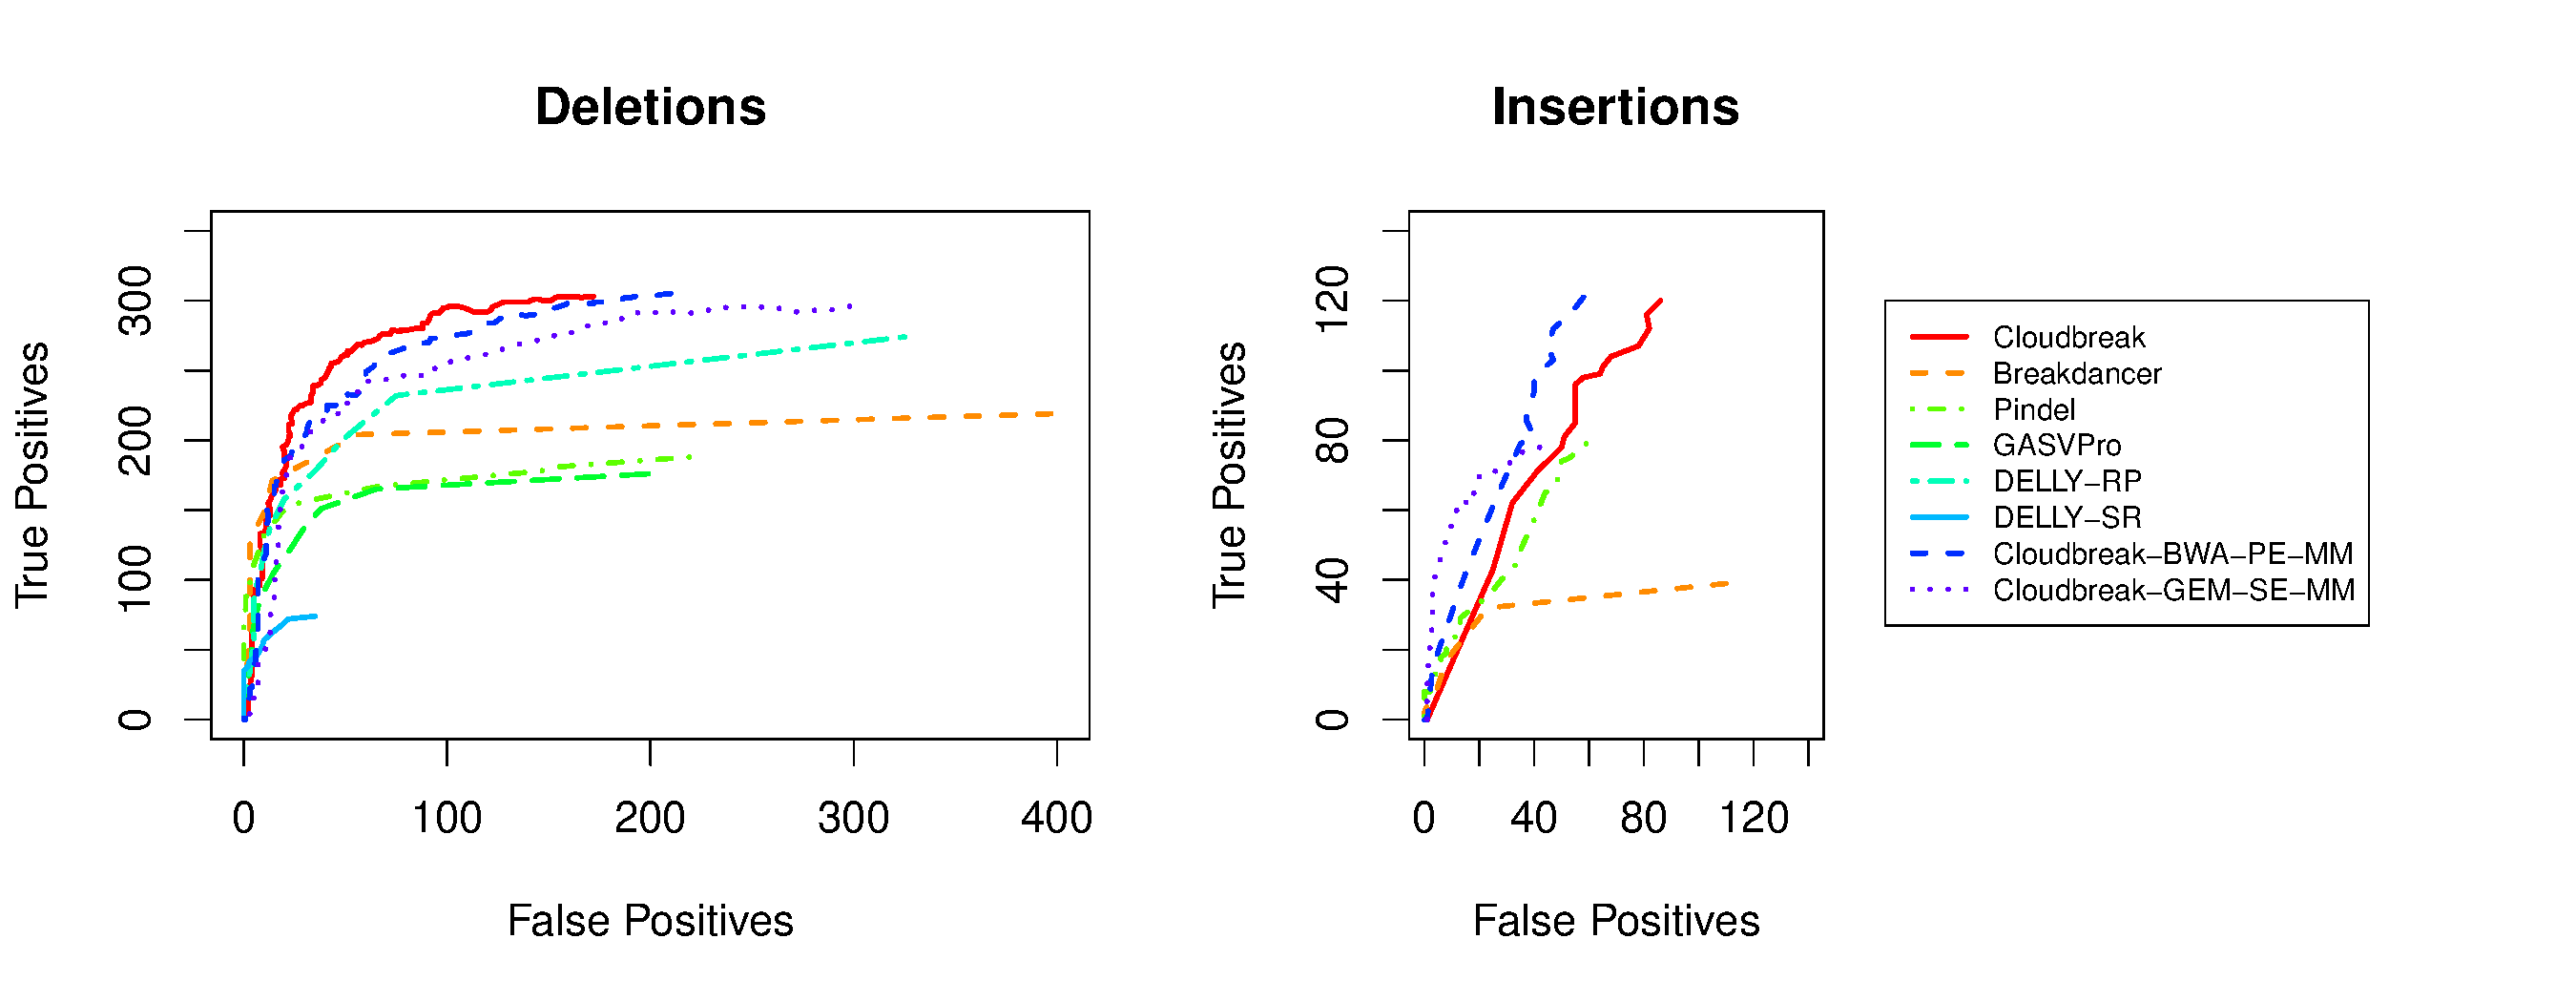
\includegraphics[width=1\textwidth]{/Users/cwhelan/Documents/svpipeline/figures/CHR2SIM_ROCS_MULTIPLE_MAPPINGS.pdf}
\caption{Cloudbreak performance on the chromosome 2 simulation using different alignment strategies. ROC curves show the number of true positives and false positives for each operating point for deletions and insertions. The Cloudbreak alignment strategies are: 1) ``Cloudbreak'': Alignments generated with BWA in paired-end mode, reporting the best hit for each pair. 2) ``Cloudbreak-BWA-PE-MM'': Alignments generated with BWA in paired-end mode, reporting up to 25 additional hits for each mapping. 3) ``Cloudbreak-GEM-SE-MM'': Alignments generated by running the GEM aligner in single-ended mode, reporting up to 1000 additional hits per alignment. Considering multiple mappings improves Cloudbreak's specificity for insertions but decreases sensitivity to deletions.}
\label{alignment_comparison}
\end{figure}

As mentioned in Section~\ref{section_incorrect_and_ambiguous_mappings}, one goal for developing Cloudbreak was to see if the use of Hadoop would allow productive use of large sets of possible mappings for ambiguously mapped read pairs. Therefore, we also tested the effect of using different aligners and including multiple mappings for ambiguously mapped reads. In addition to the BWA paired end best alignments used in the results reported above, we also used BWA in paired end mode set to report up to 25 possible mapping locations for each ambiguously mapped read pair, as well as the GEM aligner run in single ended mode on each read in each pair and set to report up to 1000 additional mappings per read. Interestingly, we found that including multiple mappings increases accuracy on insertions, but decreases performance for deletions (Figure~\ref{alignment_comparison}). This seems to indicate that while BWA's paired end mode is very good at picking correct alignments for pairs that map with long implied insert sizes, it seems to not be as good at finding correct pairings for the shorter distances indicative of insertions. We also examined the ability of all of the approaches, including Cloudbreak using both the BWA unambiguous best alignments and the GEM alignments, to detect events in repetitive regions of the genome, as shown in Table~\ref{predsByRepmask}. We found that all of the tested methods detected a similar proportion of such variants, although we did find that when used with the GEM multiple mappings, Cloudbreak does exclusively find a set of both deletion and insertion variants. In terms of runtime, use of the large set of multiple mappings did not change elapsed time to run the simulated data sample greatly, taking 308 seconds versus the 290 sections reported in the previous section. For the NA18507 dataset, the difference in runtime was more substantial, with Cloudbreak moving from taking 824 seconds to process the best alignments to 2,310 seconds to process the multiple mappings data set, a runtime which is still almost 50\% less than the next fastest approach, BreakDancer parallelized by chromosome. Although the runtimes were very manageable, we see no substantial benefit in terms of accuracy in using large sets of ambiguous mappings, at least in our current implementation.

\begin{table}
\begin{center}
\begin{tabular}{r|r|rr|rr}
  \cline{2-6}
 & & \multicolumn{2}{c}{Simulated Data} & \multicolumn{2}{c}{NA18507} \\
\hline
 & & Non-repeat & Repeat  & Non-repeat & Repeat \\ 
\multirow{9}{*}{\begin{sideways}Deletions\end{sideways}} & Total Number & 120 & 327 & 562 & 8059 \\ 
  \cline{2-6}
&  Cloudbreak  & 62 (0) & \textbf{241} (3) & \textbf{300} (\textbf{44}) & \textbf{1166} (\textbf{150}) \\ 
&  Cloudbreak-GEM  & 65 (2) & 230 (4) & 226 (8) & 1001 (17) \\ 
&  BreakDancer & 42 (0) & 177 (0) & 192 (11) & 868 (20) \\
&  GASVPro     & 37 (1) & 156 (1) & 79 (6) & 330 (16) \\
&  DELLY-RP       & 57 (1) & 217 (2) & 152 (4) & 712 (3) \\
&  DELLY-SR       & 3 (0) & 71 (0) & 27 (0) & 391 (0) \\
&  Pindel      & 26 (4) & 162 (7) & 109 (2) & 536 (6) \\ 
&  MoDIL      & \textbf{72} (\textbf{12}) & 223 (\textbf{16}) & NA & NA \\ 
   \hline
\multirow{6}{*}{\begin{sideways}Insertions\end{sideways}} & Total Number & 133 & 270 & 341 & 355 \\ 
\cline{2-6}
&  Cloudbreak  & \textbf{32} (7) & \textbf{91} (\textbf{30}) & \textbf{169} (\textbf{41}) & \textbf{148} (\textbf{43}) \\ 
&  Cloudbreak-GEM  & 21 (0) & 58 (7) & 137 (30) & 135 (32) \\ 
&  Breakdancer & 17 (5) & 22 (3) & 82 (22) & 44 (8) \\
&  Pindel      & 25 (\textbf{16}) & 54 (26) & 84 (13) & 82 (15) \\ 
&  MoDIL      & 5 (0) & 16 (2) & NA & NA \\ 
\hline
\end{tabular}
\end{center}
\caption{Detected deletions and insertions on the simulated and NA18507 data sets identified by each tool, broken down by whether the deletion overlaps with a RepeatMasker-annotated element. For all calls the maximum sensitivity cutoff was used.}
\label{predsByRepmask}
\end{table}

\section{Discussion}

We have demonstrated the Cloudbreak can deliver excellent accuracy at identifying regions that contain deletion and insertion SVs while at the same time achieving dramatically faster runtimes than other approaches through the use of the Hadoop framework and its implementation of parallel computing with data locality. In particular, the algorithm we developed for Cloudbreak is better able to identify small variants (50bp-150bp) than other tools. The downside to Cloudbreak's performance on our evaluations is its poor breakpoint resolution. As we mentioned previously, we believe that in most cases, predictions from SV detection tools require further validation, either through wet lab techniques or by further computational validation through techniques such as the split-read refinement offered by tools like DELLY, or through breakpoint assembly techniques such as TIGRA~\cite{Chen:2013gf}. In the next chapter, we will demonstrate an additional technique that improves Cloudbreak's resolution: a discriminative machine learning framework that can identify breakpoint locations by integrating read pairing, depth of coverage, and split read signals from sequencing data sets.